\everymath{\displaystyle}
\documentclass{beamer}
% \documentclass[handout]{beamer}

%\usepackage[pdftex]{color,graphicx}
\usepackage{amsmath,amssymb,amsfonts}

\mode<presentation>
{
  % \usetheme{Darmstadt}
  % \usetheme[hideothersubsections]{Hannover}
  % \usetheme[hideothersubsections]{Goettingen}
  \usetheme[hideothersubsections, right]{Berkeley}

  \usecolortheme{seahorse}
  % \usecolortheme{dolphin}
  \usecolortheme{rose}
  % \usecolortheme{orchid}

  \useinnertheme[shadow]{rounded}

  \setbeamercovered{transparent}
  % \setbeamercovered{invisible}
  % or whatever (possibly just delete it)
}

\mode<handout>{
  \setbeamercolor{background canvas}{bg=black!5}
  \usepackage{pgfpages}
  \pgfpagesuselayout{4 on 1}[a4paper,border shrink=5mm, landscape]
}

\usepackage[brazilian]{babel}
% or whatever

% \usepackage[latin1]{inputenc}
\usepackage[utf8]{inputenc}
% or whatever

\usepackage{times}
%\usepackage[T1]{fontenc}
% Or whatever. Note that the encoding and the font should match. If T1
% does not look nice, try deleting the line with the fontenc.


\title%[] % (optional, use only with long paper titles)
{Variabilidade}

\subtitle
{Incertezas de dados numéricos} % (optional)

\author%[] % (optional, use only with lots of authors)
{Felipe Figueiredo}% \and S.~Another\inst{2}}
% - Use the \inst{?} command only if the authors have different
%   affiliation.

\institute[] % (optional, but mostly needed)
{
}
  % \inst{1}%
  % Department of Computer Science\\
  % University of Somewhere
  % \and
  % \inst{2}%
  % Department of Theoretical Philosophy\\
  % University of Elsewhere}
% - Use the \inst command only if there are several affiliations.
% - Keep it simple, no one is interested in your street address.

\date%[] % (optional)
{}

% \subject{Talks}
% This is only inserted into the PDF information catalog. Can be left
% out. 



% If you have a file called "university-logo-filename.xxx", where xxx
% is a graphic format that can be processed by latex or pdflatex,
% resp., then you can add a logo as follows:

\pgfdeclareimage[height=1.6cm]{university-logo}{../logo}
\logo{\pgfuseimage{university-logo}}



% Delete this, if you do not want the table of contents to pop up at
% the beginning of each subsection:
\AtBeginSubsection[]
%\AtBeginSection[]
{
  \begin{frame}<beamer>{Sumário}
    \tableofcontents[currentsection,currentsubsection]
  \end{frame}
}


% If you wish to uncover everything in a step-wise fashion, uncomment
% the following command: 

% \beamerdefaultoverlayspecification{<+->}

\usepackage[normalem]{ulem}

\begin{document}

\begin{frame}
  \titlepage
\end{frame}

\begin{frame}{Sumário}
  \tableofcontents
  % You might wish to add the option [pausesections]
\end{frame}


%% Template
% \section{}

% \subsection{}

% \begin{frame}{}
%   \begin{itemize}
%   \item 
%   \end{itemize}
% \end{frame}

% \begin{frame}
%   \begin{columns}
%     \begin{column}{5cm}
%     \end{column}
%     \begin{column}{5cm}
%     \end{column}
%   \end{columns}
% \end{frame}

% \begin{frame}{}
%   \includegraphics[height=0.4\textheight]{file1}
%   \includegraphics[height=0.4\textheight]{file2}
%   \includegraphics[height=0.4\textheight]{file3}
%   \begin{figure}
%     \caption{}
%   \end{figure}
% \end{frame}

% \begin{frame}{}
%   \begin{definition}
%   \end{definition}
%   \begin{example}
%   \end{example}
%   \begin{block}{Exercício}
%   \end{block}
% \end{frame}

% \section{Discussão da aula passada}

% \subsection{Discussão da aula passada}

\begin{frame}{\scriptsize Discussão da aula passada}
  \begin{block}{}
    \footnotesize
    Discussão da leitura obrigatória da aula passada
  \end{block}
\end{frame}

\section{Variabilidade de dados numéricos}

\begin{frame}{\scriptsize Exemplo}
  \begin{center}
    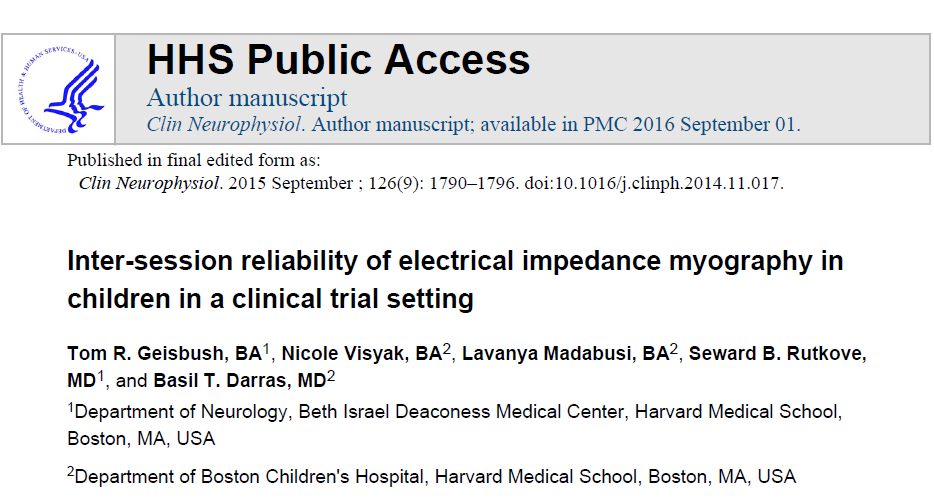
\includegraphics[width=1.2\textwidth]{Cap3/DP1}
  \end{center}
\end{frame}

% \begin{frame}{\scriptsize Abstract}
%   \begin{center}
%     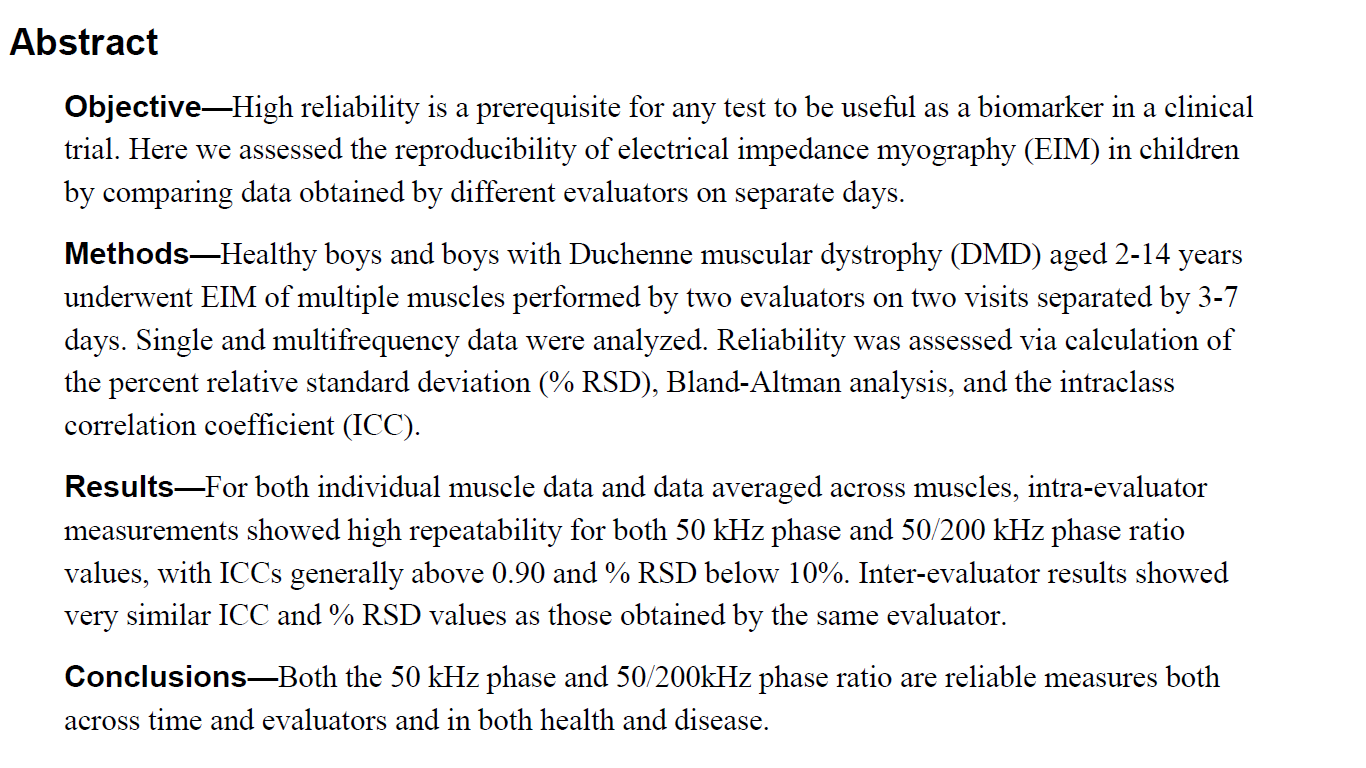
\includegraphics[width=1.2\textwidth]{Cap3/RSD-abs}
%   \end{center}
% \end{frame}

\begin{frame}[label=oquee]{\scriptsize Pergunta}
  \begin{block}{}
    \Large\centering
    O que é o desvio padrão de uma amostra?
  \end{block}
\end{frame}

\begin{frame}{\scriptsize Objetivo}
  \begin{center}
    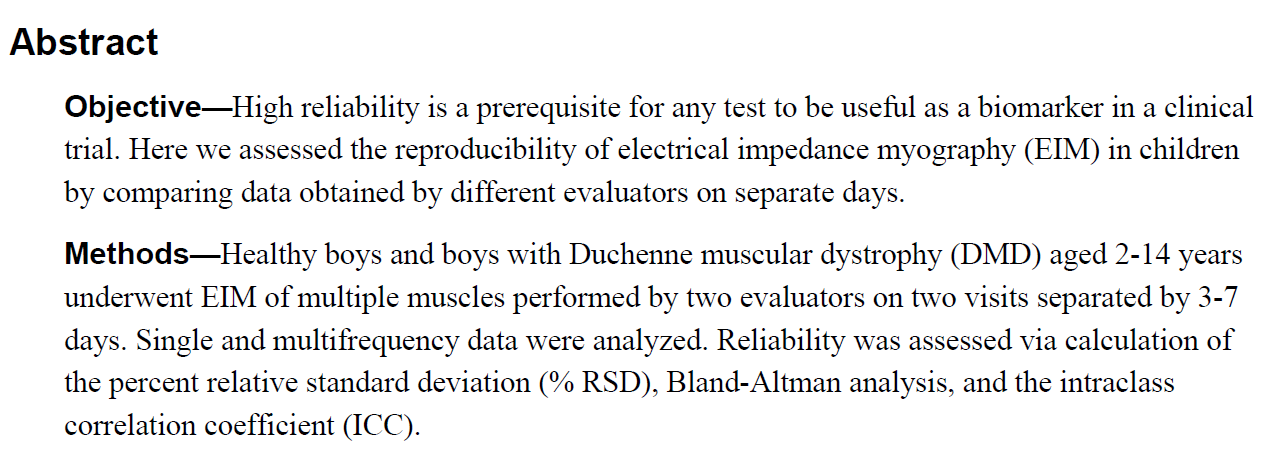
\includegraphics[width=1.2\textwidth]{Cap3/RSD0}
  \end{center}
\end{frame}

\begin{frame}{\scriptsize Desvio padrão?}
  \begin{center}
    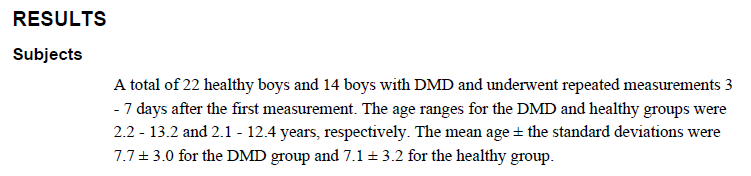
\includegraphics[width=1\textwidth]{Cap3/DP2}
  \end{center}

  \begin{block}{}
    \footnotesize
    A idade média $\pm$ desvio padrão do grupo DMD é 7.7 $\pm$ 3.0.

    \begin{itemize}
      \footnotesize
    \item O que significa este 3.0?
      \medskip
    \item Como estas descrições se comparam com as do grupo controle?
      \medskip
    \item \alert{Os grupos têm medidas médias diferentes?}
      \medskip
    \item \alert{Os grupos têm variabilidades diferentes?}
      \medskip
    \item Que outras informações você precisa para responder?
    \end{itemize}
  \end{block}
\end{frame}

\begin{frame}{\scriptsize Medidas Sumárias}
  \begin{itemize}
    \footnotesize
  \item<1,4> Medidas sumárias resumem a informação contida nos dados em um
    pequeno conjunto de números.
    \bigskip
  \item<2,3> Medidas sumárias de \alert{populações} se chamam
    \alert{parâmetros}, e são representadas por letras gregas ($\mu$, $\sigma^2$, $\sigma$, etc).
    \bigskip
  \item<3> Medidas sumárias de \alert{amostras} se chamam \alert{estatísticas} e são representadas por letras comuns ($\bar{x}$, $s^2$, $s$, etc).
    \bigskip
  \item<4> {\em Geralmente trabalhamos com estatísticas descritivas.}
  \end{itemize}
\end{frame}

\begin{frame}{\scriptsize Medidas Sumárias}
  \begin{block}{Tipos de medidas sumárias}
    \footnotesize
    Os dois principais tipos de medidas sumárias utilizadas na literatura são:
    \begin{itemize}
    \footnotesize
    \item Medidas de Tendência Central
    \item Medidas de Variabilidade (ou Dispersão)
    \end{itemize}
    \bigskip
    \hfill \scriptsize Veremos hoje ambas, com foco na Variabilidade
  \end{block}
\end{frame}

\subsection{Fontes de Variabilidade}

\begin{frame}{\scriptsize Variabilidade em Medições}
  \begin{figure}
    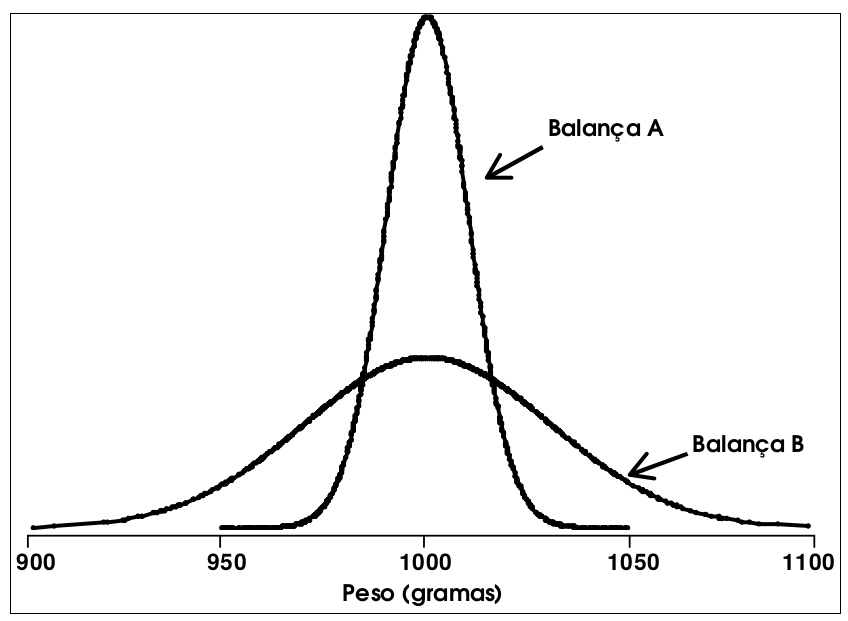
\includegraphics[height=0.7\textheight]{Cap3/variancia}
    \caption{\scriptsize Variabilidade da medição de uma esfera metálica de
      1000g. Balança A, ``imprecisão'' de 50g, balança B,
      ``imprecisão'' de 100g (Fonte: Reis, Reis, 2002)}
  \end{figure}
\end{frame}

\begin{frame}{\scriptsize Fontes comuns de variabilidade}
  \begin{itemize}
    \footnotesize
  \item Imprecisão ou erro experimental
  \item Variabilidade biológica
  \item ``{\em Mancadas}'' experimentais
  \end{itemize}
  \begin{block}{Conceito de Erro na Estatística}
    \footnotesize
    No contexto acadêmico, {\bf erro} não tem o mesmo significado do cotidiano.

    \bigskip
    Erro se refere a todas as fontes de variabilidade acima.

    \bigskip
    Outro nome comum é {\bf dispersão} ({\em scatter}).
  \end{block}
\end{frame}

\subsection{Visualizando a variabilidade com histogramas}

\begin{frame}
  \begin{exampleblock}{Exemplo}
    \footnotesize
    100 estudantes de [{\em insira aqui um curso da área da saúde}] trabalharam em pares, e mediram a pressão sistólica de seu parceiro(a).

    Ao final do exercício, a turma obteve 100 valores de pressão sistólica.
  \end{exampleblock}
  \begin{block}{Pergunta}
    \footnotesize
    Como ``entender'' essa listagem de 100 números?
  \end{block}
\end{frame}

\begin{frame}{\scriptsize O histograma}
  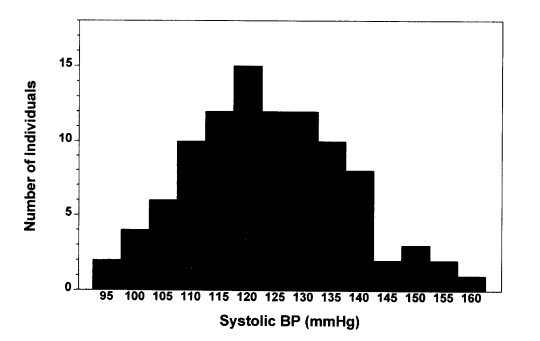
\includegraphics[height=\textheight]{Cap3/histograma1}
\end{frame}

\begin{frame}{\scriptsize Quantas barras?}
  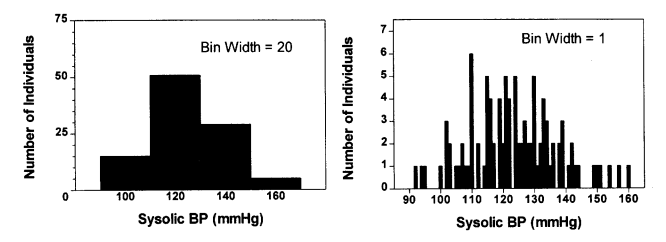
\includegraphics[width=\textwidth]{Cap3/histograma2}
\end{frame}

\subsection{Média e a mediana}

\begin{frame}{\scriptsize Média}
  \begin{exampleblock}{Exemplo 1}
    \footnotesize
    Foram observados os seguintes níveis de colesterol de uma amostra
    de pacientes. Qual é o nível médio de colesterol nestes pacientes?

    \bigskip
    \begin{columns}<1>
      \begin{column}{5cm}<1>
        {\tiny
        \begin{tabular}{ccc}
          $x_1$ &=&144\\
          $x_2$ &=&146\\
          $x_3$ &=&139\\
          $x_4$ &=&155\\
          $x_5$ &=&144\\
          $x_6$ &=&148\\
        \end{tabular}
        }
      \end{column}
      \begin{column}{5cm}<1>
        \scriptsize
        $\bar{x} = \frac{876}{6} = 146 $
      \end{column}
    \end{columns}
  \end{exampleblock}
\end{frame}

\begin{frame}{\scriptsize Percentis e a Mediana}
  \begin{block}{}
    \footnotesize
    A mediana é o dado que ocupa o percentil de 50\% dados

    (\alert{posição central}).
  \end{block}
  \bigskip
  \begin{itemize}
    \footnotesize
  \item Para se calcular a mediana, deve-se ordenar os dados.
  \item Encontrar o valor do \alert{meio} se $n$ for ímpar.
  \item Encontrar a média dos dois valores do \alert{meio} se $n$ for par.
  \end{itemize}
  % \begin{itemize}
  % \item Notação: $M_d$
  % \item Divide o dataset ao meio
  % % \item Mais robusta que a média na presença de {\it outliers}
  % \item Costuma pertencer ao dataset
  % \end{itemize}
\end{frame}

\begin{frame}{\scriptsize Mediana}
  \begin{exampleblock}{Exemplo 1}
    \footnotesize
    Conforme no exemplo (colesterol)
    \bigskip
    \tiny
    \begin{columns}
      \begin{column}{5cm}
        \begin{tabular}{ccc}
          $x_3$ &=&139\\
          $x_1$ &=&144\\
          $x_5$ &=&\alert{144}\\
          $x_2$ &=&\alert{146}\\
          $x_6$ &=&148\\
          $x_4$ &=&155\\
        \end{tabular}
      \end{column}
      \begin{column}{5cm}
        \scriptsize
        $M_d = \frac{144+146}{2}=145$
      \end{column}
    \end{columns}
  \end{exampleblock}
\end{frame}

\begin{frame}{\scriptsize }
  \begin{block}{}
    \begin{center}
      O que acontece...

      \bigskip
      ... na presença de valores extremos?
    \end{center}
  \end{block}
\end{frame}

\begin{frame}[fragile]{\scriptsize Qual é a diferença?}
  \begin{block}{}
    \footnotesize
    O que acontece com a média, na presença de um valor extremo (muito grande, ou muito pequeno em relação aos outros)?
  \end{block}
  \visible<2->{
  \begin{exampleblock}{Exemplo 1 (colesterol)}
    \bigskip
    \tiny
    \begin{columns}
      \begin{column}{5cm}
        \begin{tabular}{ccc}
          $x_1$ &=&144\\
          $x_2$ &=&146\\
          $x_3$ &=&\alert{\sout{139} = 13}\\
          $x_4$ &=&155\\
          $x_5$ &=&144\\
          $x_6$ &=&148\\
        \end{tabular}
      \end{column}
      \begin{column}{5cm}
        \scriptsize
        O que acontece se você digitar

        \alert{\bf 13} ao invés de \alert{\bf 139}?

        \bigskip
        \begin{itemize}
          \scriptsize
        \item \sout{$\bar{x} = 146, M_d= 145$}
          \medskip
        \item {\bf $\bar{x} = 125, M_d = 145$}
        \end{itemize}
      \end{column}
    \end{columns}
  \end{exampleblock}
  }\visible<3->{
  \begin{block}{Pense...}
    \scriptsize
    {\bf Qual é a implicação disso em seu projeto?}
  \end{block}
  }
\end{frame}

\begin{frame}{\scriptsize Dados corretos vs dados com outlier}
  \begin{columns}
    \begin{column}{5cm}
      \begin{center}
        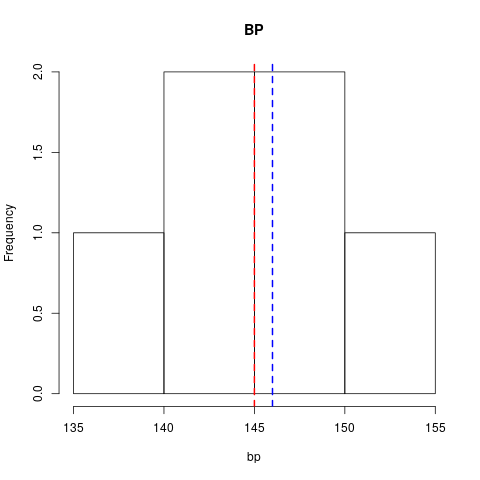
\includegraphics[width=\textwidth]{Cap3/histograma-bp}

        \scriptsize
        \bigskip
        $\bar{x} = 146 ; M_d= 145$
      \end{center}

    \end{column}
    \begin{column}{5cm}
      \begin{center}
        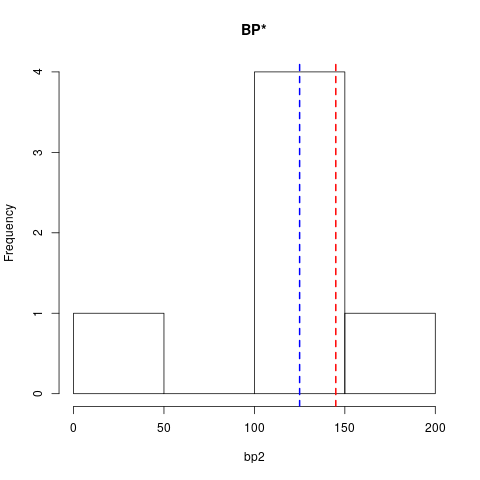
\includegraphics[width=\textwidth]{Cap3/histograma-bp2}

        \scriptsize
        \bigskip
        $\bar{x} = 125 ; M_d= 145$
      \end{center}
    \end{column}
  \end{columns}
\end{frame}

\begin{frame}{\scriptsize Medida central de dados numéricos}
  \begin{block}{Descrição de dados amostrais}
    \scriptsize
    Dados numéricos são minimamente descritos pelo seu Centro

    \bigskip
    \begin{itemize}
      \footnotesize
    \item Dados ``bem comportados''\footnote{\scriptsize paramétricos: veremos o que isso significa em aulas futuras}
      \begin{itemize}
        \scriptsize
      \item Média $\left( \bar{x} \right)$
      \end{itemize}
      \bigskip
    \item Dados ``mal comportados''
      \begin{itemize}
        \scriptsize
      \item Mediana $\left( M_d \right)$
      \end{itemize}
    \end{itemize}
  \end{block}
\end{frame}

% \begin{frame}{\scriptsize Comparação entre as Medidas Centrais}
%   \begin{exampleblock}{Exemplo}
%     \footnotesize
%     Considere o seguinte dataset $$\{ 1,1,2,4,7\}$$
%   \begin{itemize}
%     \footnotesize
%   \item $N=5$
%   \item As medidas descritivas centrais para estes dados são:
%   \item $\bar{x} = \frac{1+1+2+4+7}{5} = \frac{15}{5}= 3$
%   \item $M_d = 2$
%   \end{itemize}
% \end{exampleblock}
% \end{frame}

% \begin{frame}{\scriptsize Comparação entre as Medidas Centrais}
%   \begin{exampleblock}{Exemplo}
%     \footnotesize
%     Considere agora este outro dataset $$\{
%     1,1,2,4,\alert{32} \}$$
%   \begin{itemize}
%     \footnotesize
%   \item $N=5$
%   \item As medidas descritivas centrais para estes dados são:
%   \item $\bar{x} = \frac{1+1+2+4+32}{5} = \frac{40}{5}= 8$
%   \item $M_d = 2$
%   \end{itemize}
% \end{exampleblock}
% \end{frame}

\subsection{Quantificando com percentis}

\begin{frame}{\scriptsize Exemplo}
  \begin{center}
    
\includegraphics[height=\textheight]{Cap3/percentil0}
  \end{center}
\end{frame}

\begin{frame}{\scriptsize Exemplo}
  \begin{center}
    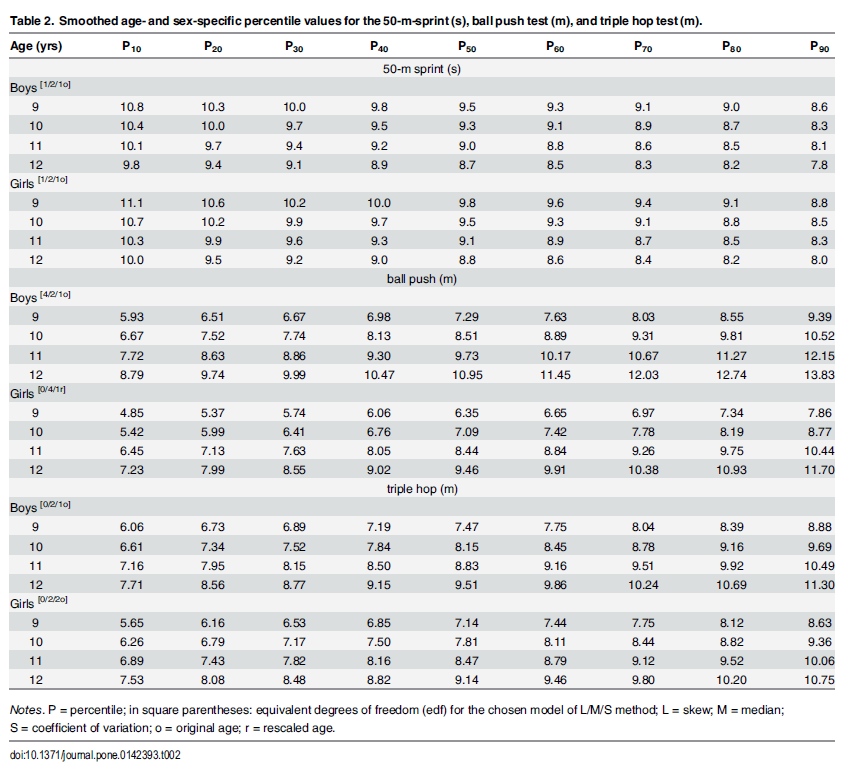
\includegraphics[height=\textheight]{Cap3/percentil1}
  \end{center}
\end{frame}

\begin{frame}{\scriptsize Exemplo}
  \begin{exampleblock}{}
    \footnotesize
    Uma criança (9 anos) faz o sprint de 50m em 10s.

    \begin{enumerate}
      \footnotesize
    \item Qual é o percentil de um menino com este tempo?
    \item Qual é o percentil de uma menina com este tempo?
    \item O que isto significa?
    \end{enumerate}
  \end{exampleblock}
  \begin{center}
    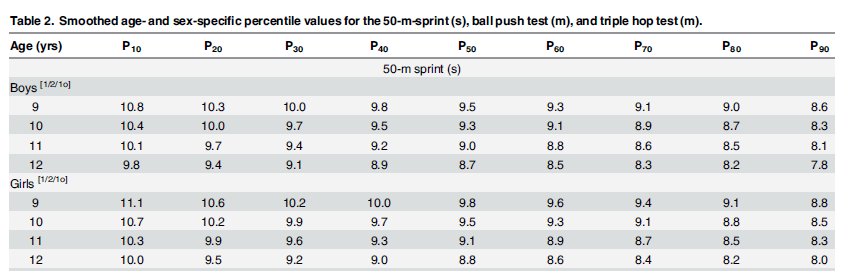
\includegraphics[width=1.2\textwidth]{Cap3/percentil2}
  \end{center}
\end{frame}

\begin{frame}{\scriptsize Medida de dispersão de dados não paramétricos}
  \begin{block}{Descrição de dados amostrais}
    \scriptsize
    Dados numéricos são suficientemente descritos por: Centro e Dispersão

    \bigskip
    \begin{itemize}
      \footnotesize
    \item Dados ``bem comportados''\footnote{\tiny Paramétricos: veremos o que isso significa em aulas futuras}
      \begin{itemize}
        \scriptsize
      \item Média (DP)
      % \item Média (Erro Padrão da Média) $\Rightarrow \bar{x} \pm$ SEM\footnote{\tiny Obs: SEM (em inglês) é uma medida inferencial e não descritiva}
      \end{itemize}
      \bigskip
    \item Dados ``mal comportados''
      \begin{itemize}
        \scriptsize
      \item Mediana e Amplitude Inter Quartílica ($M_d$ e AIQ)
      \item Mediana e Intervalo Inter Quartílico ($M_d$ e IQR {\tiny em inglês})
      \end{itemize}
    \end{itemize}
  \end{block}
\end{frame}

\begin{frame}{\scriptsize O boxplot}
  \begin{columns}
    \begin{column}{7cm}
      \begin{itemize}
        \scriptsize
      \item {\em ``Caixa e bigodes''}
        \medskip
      \item A caixa delimita os quartis de $Q_1$ e $Q_3$ ({\bf IQR})
        \begin{itemize}
          \scriptsize
        \item Percentis 25\% e 75\%
        \item O tamanho da caixa representa a {\bf AIQ}
        \end{itemize}
      \item Barra interna que representa a mediana
        \begin{itemize}
          \scriptsize
        \item Segundo quartil ($Q_2$) ou percentil de 50\%
        \end{itemize}
        \medskip
      \item Barras verticais {\em indicam} a amplitude dos dados
        \begin{itemize}
          \scriptsize
        \item Mínimo e Máximo ``razoáveis''
        \item Regras para ``a maioria''
        \end{itemize}
      \end{itemize}
    \end{column}
    \begin{column}{5cm}
      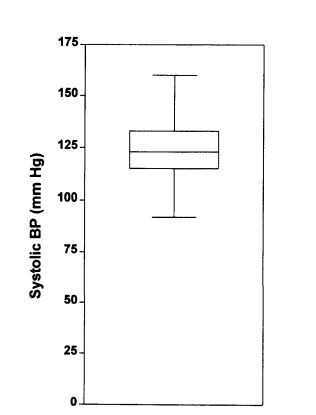
\includegraphics[height=\textheight]{Cap3/boxplot}
    \end{column}
  \end{columns}
\end{frame}

\begin{frame}{\scriptsize ``Regras para a maioria''}
  \begin{figure}
    \centering
    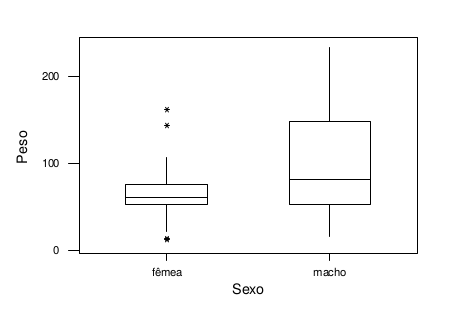
\includegraphics[height=0.7\textheight]{Cap3/boxplot3}
    \caption{\scriptsize Boxplots para dois grupos de dados (Fonte: Reis, Reis,
      2002)}
  \end{figure}
\end{frame}

\subsection{Quantificando com variância e DP}

\begin{frame}{\scriptsize A seguir, você verá...}
  \begin{columns}
    \begin{column}{5cm}
      \begin{itemize}
        \scriptsize
      \item uma cadência de ideias

        (todas relacionadas)
        \bigskip
      \item o que uma significa...

        ... em relação à próxima.
        \bigskip
      \item prós e contras de cada uma
        \bigskip
      \item do mais \alert{simples}...

        ... ao mais \alert{aplicado}.
      \end{itemize}
    \end{column}
    \begin{column}{5cm}
      \visible<2>{
        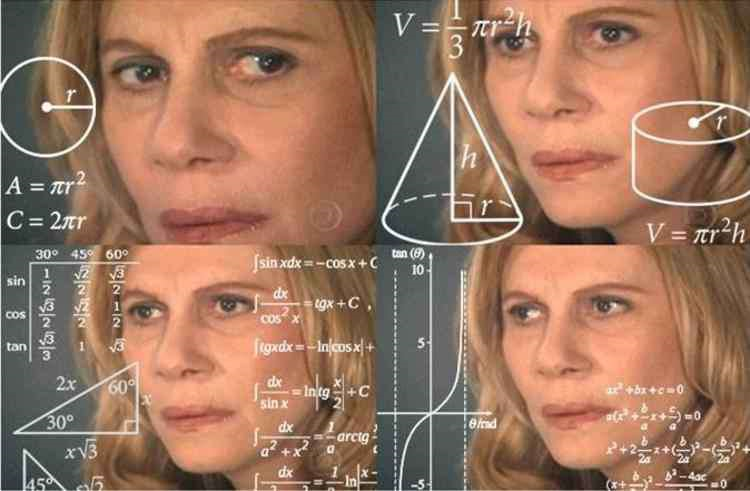
\includegraphics[width=\textwidth]{Cap3/meme-calculos2}
      }
    \end{column}
  \end{columns}
\end{frame}

\begin{frame}[label=objetivo]{\scriptsize Tenha em mente...}
  \begin{center}
    Nosso objetivo é {\bf entender}...

    \bigskip
    {\footnotesize
      ... uma medida que descreva a variabilidade de uma amostra
    }
  \end{center}
\end{frame}

\begin{frame}{\scriptsize Desvios em relação à média}
  \begin{itemize}
    \footnotesize
  \item Uma maneira de entender a variabilidade do dataset é analisar
    os desvios em relação à média.
    \bigskip
  \item Cada desvio é a diferença entre o valor do dado e a média.
  % \item $D_j = x_j - \bar{x}$ ou $D_i = x_i - \bar{x}$
  \end{itemize}
\end{frame}

\begin{frame}[fragile]{\scriptsize Dados}
  \begin{exampleblock}{\scriptsize Colesterol (N = 6, média 146)}
    \begin{center}
    \tiny
\begin{verbatim}
144 146 139 155 144 148
\end{verbatim}
    \bigskip
    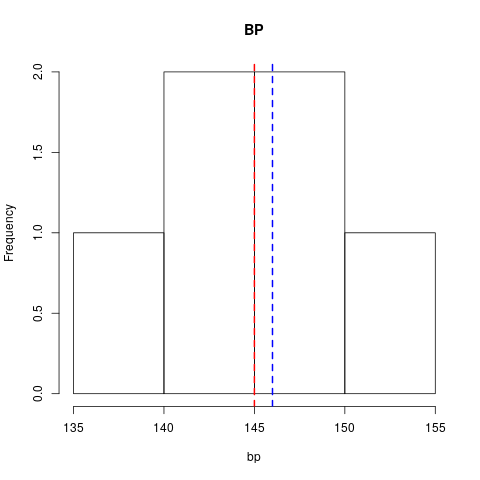
\includegraphics[height=.5\textheight]{Cap3/histograma-bp}
  \end{center}
\end{exampleblock}
  % \begin{exampleblock}{\scriptsize Distribuição dos dados}
  %   \begin{center}
  %   \end{center}
  % \end{exampleblock}
\end{frame}

\begin{frame}{\scriptsize Desvios em relação à média}
\begin{exampleblock}{Exemplo}
    \scriptsize
  \begin{displaymath}
    \{144, 146, 139, 155, 144, 148\}
  \end{displaymath}
  \bigskip
  \begin{columns}
    \begin{column}{5cm}
  \begin{itemize}
    \scriptsize
  \item $N=6$
  \item $\bar{x} = 146$
  \end{itemize}
\end{column}
\begin{column}{5cm}
  \begin{enumerate}
    \tiny
  \item $D_1 = 144 - 146 = -2$
  \item $D_2 = 146 - 146 = 0$
  \item $D_3 = 139 - 146 = -7$
  \item $D_4 = 155 - 146 = 9$
  \item $D_5 = 144 - 146 = -2$
  \item $D_6 = 148 - 146 = 2$
  \end{enumerate}
\end{column}
\end{columns}
\end{exampleblock}
\end{frame}

\begin{frame}[fragile]{\scriptsize Desvios em relação à média}
  \begin{block}{Colesterol (N = 6, média 146)}
    \footnotesize
\begin{verbatim}
144 146 139 155 144 148
\end{verbatim}
  \end{block}
  \begin{block}{Desvios em relação à média}
    \footnotesize
\begin{verbatim}
-2  0 -7  9 -2  2
\end{verbatim}
  \end{block}
\end{frame}

\begin{frame}{\scriptsize Desvios em relação à média}
  \footnotesize
  Mas os desvios...
  \bigskip
  \begin{enumerate}
    \footnotesize
  \item são tão numerosos quanto os dados
    \bigskip
  \item têm sinal (direção do desvio)
    \bigskip
  \item SEMPRE têm soma \alert{nula}, portanto o desvio médio é sempre 0
  \end{enumerate}
  \bigskip
  \vfill
  \begin{block}{Pense...}
    \footnotesize
    Uma fórmula que dá o mesmo resultado para qualquer dataset... serve para resumir seus dados?
  \end{block}
\end{frame}

\begin{frame}{\scriptsize Soma dos desvios}
  \begin{exampleblock}{Exemplo}
    \footnotesize
    Somando tudo:
    \begin{displaymath}
    \sum D = D_1 + D_2 + D_3 + D_4 + D_5 + D_6 =
  \end{displaymath}
  \begin{displaymath}
    (-2) + 0 + (-7) + 9 + (-2) + 2 = \alert{0}
  \end{displaymath}
  \end{exampleblock}
  \bigskip
  \vfill
  \begin{block}{Pense...}
    \footnotesize
    Uma fórmula que dá o mesmo resultado para qualquer dataset... serve para resumir seus dados?
  \end{block}
\end{frame}

\begin{frame}{\scriptsize Como proceder?}
  \begin{itemize}
    \footnotesize
  \item Como extrair alguma informação útil (e sumária!) dos desvios?
  \item Problema: sinais
  \end{itemize}
  \bigskip
  \vfill
  \begin{block}{Pergunta}
    \footnotesize
    Como tirar os sinais dos desvios?
    \visible<2>{
    \begin{block}{}
      \begin{enumerate}
        \scriptsize
      \item Tirar o módulo (valor absoluto)
      \item Elevar ao quadrado
      \end{enumerate}
    \end{block}
    }
  \end{block}
\end{frame}

\begin{frame}{\scriptsize Desvios absolutos}
  \scriptsize
  Tomando-se o módulo dos desvios temos:
  % \item Idéia matemática de ``tamanho''

  \bigskip
  \begin{block}{Definição}
    \footnotesize
    Desvio médio absoluto (MAD) é a média dos desvios absolutos
  \end{block}

  \bigskip
  \begin{itemize}
    \scriptsize
  \item É uma medida de dispersão robusta (pouco influenciada por
    outliers)
    \medskip
  \item Módulo não tem boas propriedades matemáticas (analíticas e
    algébricas).
    \medskip
  \item Pouco usado para inferência (apesar da robustez)
  \end{itemize}
\end{frame}

\begin{frame}{\scriptsize Desvio médio absoluto (MAD)}
  \begin{exampleblock}{Exemplo}
    \footnotesize
  \begin{displaymath}
    \{144, 146, 139, 155, 144, 148\}, \bar{x} = 146
  \end{displaymath}
  \begin{columns}
    \begin{column}{5cm}<1->
      \begin{enumerate}
        \tiny
      \item $|D_1| = |144 - 146| = 2$
      \item $|D_2| = |146 - 146| = 0$
      \item $|D_3| = |139 - 146| = 7$
      \item $|D_4| = |155 - 146| = 9$
      \item $|D_5| = |144 - 146| = 2$
      \item $|D_6| = |148 - 146| = 2$
      \end{enumerate}
    \end{column}
    \begin{column}{5cm}
      \begin{displaymath}
        \mathrm{MAD} = \frac{\sum |D_i|}{6} = 3.7
      \end{displaymath}
    \end{column}
  \end{columns}
\end{exampleblock}
% \begin{block}{No exemplo do paper}
%     \footnotesize
%   MAD = 3.24
% \end{block}
\end{frame}

\begin{frame}{\scriptsize Uma proposta ``melhor''}
  \begin{itemize}
    \footnotesize
  \item Uma outra maneira de eliminar os sinais é elevar ao quadrado
    cada desvio.
    \bigskip
  \item Preserva boas propriedades matemáticas
    \bigskip
  \item Calculando a média dos quadrados dos desvios (desvios
    quadráticos) temos \ldots
  \end{itemize}
\end{frame}

\begin{frame}{\scriptsize Variância}
  \begin{block}{Definição}
    A variância é a média dos desvios quadráticos.
  \end{block}
  \begin{itemize}
    \footnotesize
  \item Variância populacional
$$\sigma^2 = \frac{\sum (x_j - \mu)^2}{N}$$
\item Variância amostral
$$s^2 = \frac{\sum (x_i - \bar{x})^2}{n-1}$$
\item Conveniente do ponto de vista matemático (boas propriedades
  algébricas e analíticas).
\item Unidade quadrática, pouco intuitiva para interpretação de
  resultados.
  \end{itemize}
\end{frame}

\begin{frame}{\scriptsize Variância}
  \begin{exampleblock}{Exemplo}
    \scriptsize
      \begin{displaymath}
    \{144, 146, 139, 155, 144, 148\}, \bar{x} = 146
  \end{displaymath}
    \bigskip
    \tiny
  \begin{columns}
    \begin{column}{6cm}<1->
      \begin{enumerate}
        \tiny
      \item $(D_1)^2 = (144-146)^2 = (-2)^2 = 4$
      \item $(D_2)^2 = (146-146)^2 = 0^2 = 0$
      \item $(D_3)^2 = (139-146)^2 = (-7)^2 = 49$
      \item $(D_4)^2 = (155-146)^2 = 9^2 = 81$
      \item $(D_5)^2 = (144-146)^2 = (-2)^2 = 4$
      \item $(D_6)^2 = (148-146)^2 = 2^2 = 4$
      \end{enumerate}
    \end{column}
    \begin{column}{4cm}
      \footnotesize
      \begin{displaymath}
        s^2 = \frac{\sum D_i^2}{5} = 28.4
      \end{displaymath}
    \end{column}
  \end{columns}
  \end{exampleblock}
  \begin{block}{No exemplo do paper}
    \scriptsize
    VAR = 18.14
  \end{block}
\end{frame}

\begin{frame}{\scriptsize Desvio Padrão}
  \begin{block}{Definição}
    O desvio padrão é a raiz quadrada da variância.
  \end{block}
  \begin{itemize}
    \footnotesize
  \item Desvio padrão populacional
    $$ \sigma = \sqrt{ \sigma^2 } = \sqrt{ \frac{\sum (x_i - \mu)^2}{N} } $$
    \bigskip
  \item Desvio padrão amostral
    $$ s = \sqrt{s^2 } = \sqrt{ \frac{\sum (x_i - \bar{x})^2}{n-1} } $$
  \end{itemize}
\end{frame}

\begin{frame}{\scriptsize Desvio Padrão}
  \begin{itemize}
    \footnotesize
  \item É a medida mais usada, por estar na mesma escala (unidade) dos
    dados.
    \bigskip
  \item Boas propriedades matemáticas
    \bigskip
  \item Boas propriedades como estimador (Inferência)
  \end{itemize}
\end{frame}

\begin{frame}{\scriptsize Desvio Padrão}
  \begin{exampleblock}{Exemplo}
    \scriptsize
      \begin{displaymath}
        \{144, 146, 139, 155, 144, 148\}, \bar{x} = 146
      \end{displaymath}
      \medskip
      \begin{displaymath}
        s^2 = 28.4
      \end{displaymath}
      \medskip
      \begin{displaymath}
        s = \sqrt{s^2} = \sqrt{28.4} = 5.3
    \end{displaymath}
  \end{exampleblock}
  \begin{block}{No exemplo do paper}
    \footnotesize
    s = 4.26
  \end{block}
\end{frame}

\begin{frame}{\scriptsize}
  \begin{block}{Lembre-se}
    \footnotesize
    Você não precisa {\bf saber fazer} esses cálculos!

    \bigskip
    Eles são feitos instantaneamente por máquinas!
  \end{block}
  \bigskip
  \vfill
  \begin{center}
    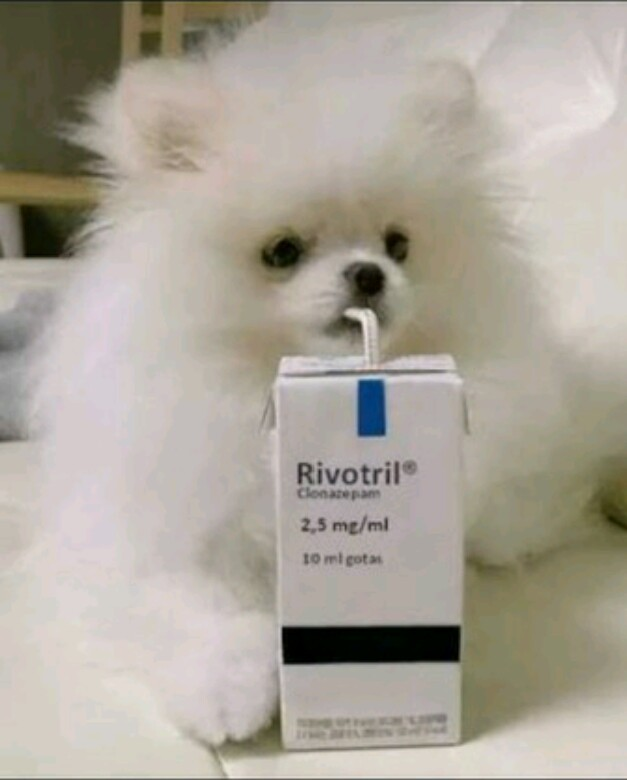
\includegraphics[height=.5\textheight]{Cap3/meme-rivis}
  \end{center}
\end{frame}

\againframe{objetivo}

\begin{frame}{\scriptsize Como comparar o DP de dois grupos?}
  \begin{block}{}
    \footnotesize
    Não podemos comparar diretamente o \alert{valor} do DP de dois grupos.

    \bigskip
    Por que?
  \end{block}
\end{frame}

\begin{frame}{\scriptsize O Desvio Padrão Relativo}
  \begin{block}{Desvio Padrão Relativo}
    \footnotesize
    O desvio padrão relativo é uma medida de dispersão \alert{normalizada}.

    \bigskip
    Ela ignora a escala da mensuração.

    $$DPR = \frac{s}{\bar{x}}\times 100$$
  \end{block}
  \begin{exampleblock}{Sinônimos}
    \footnotesize
    \begin{itemize}
    \footnotesize
    \item Desvio padrão relativo (DPR)
    \item Coeficiente de Variação (CV)
    \item {\em Relative Standard Deviation} (RSD)
  \end{itemize}
  \end{exampleblock}
\end{frame}

\begin{frame}{\scriptsize O Desvio Padrão Relativo}
  \begin{center}
    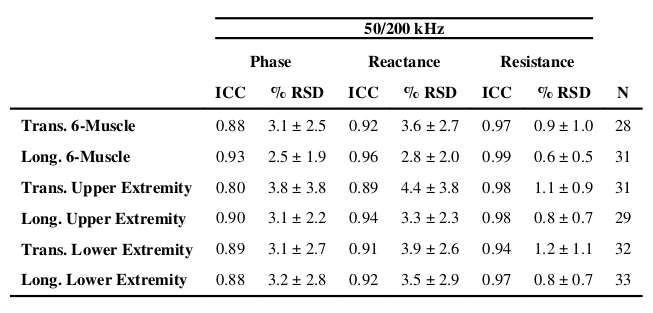
\includegraphics[width=\textwidth]{Cap3/RSD1}
  \end{center}
  \begin{exampleblock}{Dos nossos dados}
    \footnotesize
    CV = 4\%
  \end{exampleblock}
\end{frame}

\subsection{N ou N-1?}

\begin{frame}{\scriptsize N ou N-1?}
  \begin{block}{Fórmula com N}
    \footnotesize
    Usada apenas para cálculos com dados de toda a população.
  \end{block}
  \begin{block}{Fórmula com N-1}
    \footnotesize
    Usada para cálculos com dados de uma amostra.
  \end{block}
  \begin{block}{Pense...}
    \footnotesize
      Você tem acesso a toda a população, ou apenas a uma amostra?
  \end{block}
\end{frame}

\begin{frame}{\scriptsize Quiz}
  \begin{block}{Pergunta}
    \footnotesize
    O desvio dos dados em relação à média é uma medida de dispersão:

    \bigskip
    \begin{enumerate}
      \scriptsize
    \item Verdadeiro
    \item \alert<2>{Falso}
      \invisible{
    \item 1
    \item 1
      }
    \end{enumerate}
  \end{block}
\end{frame}

\begin{frame}{\scriptsize Quiz}
  \begin{block}{Pergunta}
    \footnotesize
    São medidas adequadas para descrever o centro dos dados:

    \bigskip
    \begin{enumerate}
      \scriptsize
    \item \alert<2>{Média ($\bar{x}$)}
    \item Variância ($s^2$)
    \item Percentis
    \item \alert<2>{Mediana}
    \end{enumerate}
  \end{block}
\end{frame}

\begin{frame}{\scriptsize Quiz}
  \begin{block}{Pergunta}
    \footnotesize
    A medida de dispersão mais utilizada na prática é:

    \bigskip
    \begin{enumerate}
      \scriptsize
    \item Variância ($s^2$)
    \item Desvio Médio absoluto (MAD)
    \item \alert<2>{Desvio padrão ($s$)}
    \item Desvio padrão relativo (DPR)
    \end{enumerate}
  \end{block}
\end{frame}

\subsection{Interpretação do DP}

\begin{frame}{\scriptsize Interpretação do DP}
  \begin{block}{}
    \footnotesize
    {\em ``Um pouco mais da metade'' dos valores está a 1 DP da média (considerando ambos os lados)}
  \end{block}
  \begin{block}{}
    \footnotesize
    {\em ``Quase todos'' os dados estão a 2 DP da média (considerando ambos os lados)}
  \end{block}
  \begin{itemize}
    \footnotesize
  \item {\em Cenas dos próximos capítulos}
  \end{itemize}
\end{frame}

\againframe{oquee}

\section{Aprofundamento}

\subsection{Aprofundamento}

\begin{frame}{\scriptsize Aprofundamento}
  \begin{block}{Leitura obrigatória}
    \footnotesize
    Capítulo 3. Pular as seções:
    \begin{itemize}
      \footnotesize
    \item Calculando o DP numa calculadora
    % \item Coeficiente de Variação (CV)
    \end{itemize}
  \end{block}
  \begin{block}{Leitura recomendada}
    \scriptsize
    Não há
  \end{block}
\end{frame}

\end{document}
